% !TeX spellcheck = en_US
\documentclass[french]{yLectureNote}

\title{Atomistique}
\subtitle{La matière à l'échelle atomique}
\author{Paulhenry Saux}
\date{\today}
\yLanguage{Français}

\professor{J.Cuny}%sebastien.deveuhels.irap.omp.eu

\usepackage{graphicx}%----pour mettre des images
\usepackage[utf8]{inputenc}%---encodage
\usepackage{geometry}%---pour modifier les tailles et mettre a4paper
%\usepackage{awesomebox}%---pour les boites d'exercices, de pbq et de croquis ---d\'esactiv\'e pour les TP de PC
\usepackage{tikz}%---pour deiffner + d\'ependance de chemfig
\usepackage{tkz-tab}
\usepackage{chemfig}%---pour deiffner formules chimiques
\usepackage{chemformula}%---pour les formules chimiques en \'equation : \ch{...}
\usepackage{tabularx}%---pour dimensionner automatiquement les tableaux avec variable X
\usepackage{awesomebox}%---Pour les boites info, danger et autres
\usepackage{menukeys}%---Pour deiffner les touches de Calculatrice
\usepackage{fancyhdr}%---pour les en-t\^ete personnalis\'ees
\usepackage{blindtext}%---pour les liens
\usepackage{hyperref}%---pour les liens (\`a mettre en dernier)
\usepackage{caption}%---pour la francisation de la l\'egende table vers Tableau
\usepackage{pifont}
\usepackage{array}%---pour les tableaux
\usepackage{lipsum}
\usepackage{yFlatTable}
\usepackage{multicol}
\newcommand{\Lim}[1]{\lim\limits_{\substack{#1}}\:}
\renewcommand{\vec}{\overrightarrow}
\begin{document}
\setcounter{chapter}{1}

	\chapter{Orbitales atomiques}
\section{Équation de Schrödinger}
\subsubsection{Nombres quantiques}
Pour chaque couche n, il existe $n^2$ Orbitales atomiques. Chaque OA est caractérisée par 3 nombres quantiques : n, l et ml. Ce sont des entiers.

Une couche est l'ensemble des m\^emes OA avec le m\^eme n.
\warningInfo{Dégénrences}{2 OA sont dites degénérées si elles sont la m\^eme énergie.}

	\begin{tabular}{_l^l^l^l}
		\tableHeaderStyle%
		Nombre & Utilité & valeurs & Nombre de valeurs\\
		n & énergie/taille de l'orbitale & 1.2.3& n\\
		l & forme de l'orbitale & 0,1,2,...,(n-1)&n\\
		ml & orientation de l'orbitale & l,l-1,...,1,0,-1,...-(l-1),-l&(2l+1)\\
	\end{tabular}
\subsubsection{Nomenclature des sous-couches}
XY avec X = n et Y : Voir tableau pour la corresponde l$\rightarrow$lettre.

	\begin{tabular}{_c^c}
		\tableHeaderStyle%
		valeur de l & lettre correspondante \\
		0 & s\\
		1 & p\\
		2 & d\\
		3 & f\\
		4 & g\\
		5 & h\\
	\end{tabular}
	\subsection{Le spin}
\subsubsection{Définition}
	Il existe un 4e nombre quantique qui quantifie le moment cinétique intrinsèque, qui existe pour toute particules quantiques\marginCritical{Il ne faut pas confondre le nombre quantique de spin, le spin (=moment cinétique intrisèque) et le nombre magnétique de spin.} :
	\begin{itemize}
	 \item le nombre quantique de spin, noté s pour l'électron. Il vaut $\frac{1}{2}$. (Les fermions ont un nombre demi-entier)
	 \item le nombre quantique magnétique de spin, $m_s$, qui ne peut prendre que $2s+1$ valeurs. Il peut prendre 2 valeurs $\pm\frac{1}{2}$
	\end{itemize}
	\subsection{Règle de Pauli}
Selon Pauli, Dans la fonction d'onde, si j'inverse 2 électrons, cela génère un -.\marginInfo{Il l'a dit selon ces termes : ``La fonction d'onde d'un système fermionique est antisymétrique par permutation''}
\criticalInfo{Conséquence}{Dans l'atome, 2 électrons ne peuvent pas avoir leur 4 nombre quantique identique. Une OA ne peut donc décrire que 2 électrons}

\section{Présentation des fonctions}
\subsection{Orbitale atomique}
$\hat{H}\Psi(r,\theta,\varphi) = E\Psi(r,\theta,\varphi)$. Les orbitales atomiques sont les solutions de cette équation et s'exprime en coordonnées sphériques\marginCritical{Propriétés importantes de ces coordonnées : \begin{itemize}
 \item $\mathrm{d}v = r^2\mathrm{d}r \sin\theta \mathrm{d}\theta \mathrm{d} \varphi$
 \item $\theta : 0 \rightarrow \pi$
 \item $\varphi : 0 \rightarrow 2\pi$
\end{itemize}}.
On a : \[\Psi_{n,l,m_l} = R_{n,l}(r)Y_{l,m_l}(\theta,\varphi)\]
\subsection{Sens physique de la fonction d'onde}
	\begin{tabular}{_l^l^l}
		\tableHeaderStyle%
		Expression & Sens physique& Unité\\
		$\Psi(r,\theta,\varphi)$ & Aucun & m$^{-3/2}$ \\
		$|\Psi(r,\theta,\varphi)|^2$ &  densité de probabilité de présence de l'électron au point $r,\theta,\varphi$ & m$^{-3}$\\
		$|\Psi(r,\theta,\varphi)|^2 d\tau$ & Probabilité infinitésimale & m$^{-3}$\\
		$\int\int\int|\Psi(r,\theta,\varphi)|^2 d\tau$ & Probabilité pour un certain volume & m$^{-3}$\\
	\end{tabular}
\subsection{Condition de normalisation}
\warningInfo{Définition}{Toutes les fonctions d'onde sont normalisées car leur intégrale sur tout l'espace fait 1. Ainsi, on a : \[\int_0^{+\infty}\int_0^{\pi}\int_0^{2\pi}|\Psi(r,\theta,\varphi)|^2 d\tau = 1\] et donc \[\int_0^{+\infty}R_{n,l}(n)^2 r^2\mathrm{d}r = \int_0^{\pi}\int_0^{2\pi}|Y_{l,ml}(\theta,\varphi)|^2  \sin\theta \mathrm{d}\theta \mathrm{d} \varphi  = 1\]
}
\section{Étude des fonctions}
\subsection{Fonction radiale}



\begin{multicols}{2}
$R_{n,l}(n)^2 r^2$ est toujours nulle à l'origine. Les valeurs nulles en dehors de celle à l'origine de la fonction sont les noeuds radiaux.

Pour décrire où un électron peut se trouver, il faut utiliser $|R_{n,l}(n)|^2 r^2$ dont l'intégrale est normalisée.

\columnbreak

\includegraphics[scale=0.4]{OA-rad}

\end{multicols}
\warningInfo{Représentations}{Un minimum de $R(r)^2r^2$ indique qu'il y a un noeud radial, donc une valeur nulle sur $R(r)$ !

Cela signifie qu'en un noeud radial, la croissance de $R(r)^2r^2$ change et sa dérivée est donc nulle : Un noeud radial est donc une racine de la dérivée !}
\subsection{Partie angulaire}

On fait des combinaisons linéaires de$\pm m_l$ pour trouver des fonctions réelles que l'on peut représenter.
\criticalInfo{Conséquence}{Toutes les orbitales atomiques sont définies au signe près.}

%La partie angulaire à $l-|m|$ noeuds}


On peut déterminer la sous-couche de la représentation en déterminant le nombre de surfaces nodales présentes sur une symétrie. \marginCritical{Par exemple, sur le membre de droite des représentations des OA de type $p$, il y a une symétrie pour n=2, 2 pour n=3 et 3 pour n=4. De cette manière, on peut déterminer $n$. Pour le type $p$, il y a une symétrie pour n=3 et 2 pour n=3. }

\subsection{Sur les noeuds}
Il faut différentier les noeuds sphériques correspondant aux zéros de la fonction \emph{radiale} et les noeuds plans (donnés par la fonction \emph{angulaire}).

Le nombre de noeud sphérique est donné par $n-l-1$ et les noeuds angulaires sont donnés par $l$.

\begin{multicols}{2}
\begin{center}
 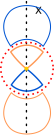
\includegraphics[scale=0.4]{noeuds}
\end{center}

\columnbreak

Sur le schéma ci-contre, représentant l'OA $3px$ le noeud rouge représente le noeud radial et le jaune le noeud angulaire.

\begin{tabular}{_c^c^c}
		\tableHeaderStyle%
		Orbitales & N. plans & N. sphériques\\
		s & 0 & n-1\\
		p & 1 & n-2\\
		d & 2 & n-3\\
	\end{tabular}


\end{multicols}
\subsection{Multiplication des 2 parties}
\begin{multicols}{2}
Lorsque l'on multiplie la partie angulaire avec la partie radiale, 2 choses se produisent :
\begin{itemize}
\item L'OA s'agrandit
\item Elle se sépare selon les points nodaux de R : un nouveau noeud sphérique apparait
\end{itemize}

Pour passer de l'OA $2p$ à l'OA $3p$, on regarde la représentation de $R_{3,1}(r)$ (Fig2.1) et on observe un noeud radial à une distance $a$.

\columnbreak

\includegraphics[scale=0.5]{3p-r}
\captionof{figure}{Some here}
\end{multicols}
On aura donc une nouvelle surface nodale sur la représentation sur  le schéma ci-dessous :

\includegraphics[scale=0.3]{2p-3p}
\section{Méthode}

\subsection{Trouver quelle formule utiliser sur la partie radiale}
 $\int_0^{+\infty} |R_{n,l}(n)|^2 r^2 dr = 1$ est utilisée pour la condition de normalisation.

 Trouver la distance électron-noyau pour laquelle la probabilité de présence est maximale. On dérive $R_{n,l}(r)^2r^2$.


\subsection{Trouver la distance électron-noyau pour laquelle la densité de probabilité de présence radiale est maximale}
\begin{enumerate}
 \item On prend la formule $R_{n,l}(r)$ de l'OA étudiée
 \item On la met au carré et on multiplie par $r^2$ : $R_{n,l}(n)^2 r^2$
 \item On dérive la fonction
 \item On factorise avec des racines évidentes ou d'autres méthodes pour trouver toutes les valeurs de $r$ où la dérivée s'annule
 \item Le maximum de probabilité est atteint pour le $r$ le plus éloigné du noyau. On classe donc les racines trouvée par taille et on prend la plus grande
\end{enumerate}

\subsection{Représenter une fonction angulaire complexe en fonction angulaire réelle}
On utilise des formules de linéarisation puis celles d'Euler\marginInfo{\[\cos(\theta) = \frac{e^{i\theta} + e^{-i\theta}}{2}\]  \[\sin(\theta) = \frac{e^{i\theta} - e^{-i\theta}}{2i}\]}

\begin{theorem}[Formule de linéarisation de la partie angulaire]
\begin{itemize}
 \item $\displaystyle S^+_{l|m|} = \frac{Y_{l,m} + Y_{l,-m}}{\sqrt{2}} $
 \item $\displaystyle S^-_{l|m|} = \frac{Y_{l,m} - Y_{l,-m}}{i\sqrt{2}} $
\end{itemize}

\end{theorem}
Exemple Pour $Y_{1,\pm1}$ :
\begin{flalign*}
S^+_{l|m|} &= \frac{Y_{l,m} + Y_{l,-m}}{\sqrt{2}}\\
&= \frac{ \frac{1}{2}(\frac{3}{2\pi})^{1/2}\sin(\theta)e^{i\varphi}  +\frac{1}{2}(\frac{3}{2\pi})^{1/2}\sin(\theta)e^{-i\varphi} }{\sqrt{2}}\\
&= \frac{ \frac{1}{2}(\frac{3}{2\pi})^{1/2}\sin(\theta)(e^{i\varphi}+ e^{-i\varphi}) }{\sqrt{2}}\\
&= \frac{ \frac{1}{2}(\frac{3}{2\pi})^{1/2}\sin(\theta)(2\cos(\varphi)) }{\sqrt{2}}\\
&= \frac{(\frac{3}{2\pi})^{1/2}\sin(\theta)(\cos(\varphi)) }{\sqrt{2}}\\
&= \frac{(\frac{3}{2\pi})^{1/2}\sin(\theta)(\cos(\varphi)) }{\sqrt{2}}\\
&= (\frac{3}{4\pi})^{1/2}\sin(\theta)(\cos(\varphi))
\end{flalign*}

\subsection{Montrer que la partie radiale est normalisée}
Il faut montrer que $\int_0^{+\infty} |R_{n,l}(n)|^2 r^2 dr = 1$

Exemple avec R de 1 et 0 :

\begin{flalign*}
\int_0^{+\infty} |R_{n,l}(n)|^2 r^2 dr &=\\
&=(\frac{Z}{a_0})^3\times 4\int_0^{+\infty} e^{-\frac{-2Zr}{a_0}} r^2 dr\\
&= (\frac{Z}{a_0})^3\times 4 \times \frac{2!}{(\frac{Z}{a_0})^3}\\
&= \frac{4\times 2}{8} = 1
\end{flalign*}

Exemple avec R de 4 et 2 :

\begin{flalign*}
\int_0^{+\infty} |R_{4,2}(n)|^2 r^2 dr &=\\
&=(\frac{Z}{a_0})^3\times \frac{1}{384^2\times 5} \int_0^{+\infty} \rho^4(6-\frac{1}{2}\rho)^2 e^{-\frac{Zr}{2a_0}} r^2 dr\\
&=(\frac{Z}{a_0})^3\times \frac{1}{384^2\times 5} \int_0^{+\infty} (\frac{Z}{a_0})^4\times r^4(36-6\rho+\frac{1}{4}\rho^2) e^{-\frac{Zr}{2a_0}} r^2 dr\\
&=(\frac{Z}{a_0})^7\times \frac{1}{384^2\times 5} \int_0^{+\infty} r^6(36-6\rho+\frac{1}{4}\rho^2) e^{-\frac{Zr}{2a_0}} dr\\
&=(\frac{Z}{a_0})^7\times \frac{1}{384^2\times 5}  \int_0^{+\infty} 36r^6e^{-\frac{Zr}{2a_0}} - 6\rho r^6e^{-\frac{Zr}{2a_0}}+\frac{1}{4}\rho^2r^6e^{-\frac{Zr}{2a_0}} dr\\
&=(\frac{Z}{a_0})^7\times \frac{1}{384^2\times 5} \times(36\int_0^{+\infty}r^6e^{-\frac{Zr}{2a_0}}dr - 6\int_0^{+\infty}\rho r^6e^{-\frac{Zr}{2a_0}}dr+\frac{1}{4}\int_0^{+\infty}\rho^2r^6e^{-\frac{Zr}{2a_0}}dr)\\
&=(\frac{Z}{a_0})^7\times \frac{1}{384^2\times 5} \times(36\int_0^{+\infty}r^6e^{-\frac{Zr}{2a_0}}dr - 6\frac{Z}{a_0}\int_0^{+\infty}r^7e^{-\frac{Zr}{2a_0}}dr+\frac{1}{4}(\frac{Z}{a_0})^2\int_0^{+\infty}r^8e^{-\frac{Zr}{2a_0}}dr)\\
&=(\frac{Z}{a_0})^7\times \frac{1}{384^2\times 5} \times(36\frac{6!}{(\frac{Z}{2a_0})^7}- 6\frac{7!}{(\frac{Z}{2a_0})^7}+\frac{1}{4}\frac{8!}{(\frac{Z}{2a_0})^7})\\
&=(\frac{Z}{a_0})^7\times \frac{1}{384^2\times 5} \times(\frac{6!}{(\frac{Z}{2a_0})^7}(36-6\times7+\frac{1}{4}\times8\times7))\\
&=(\frac{Z}{a_0})^7\times \frac{1}{384^2\times 5} \times(\frac{6!}{(\frac{Z}{2a_0})^7}(8))\\
&=(\frac{Z}{a_0})^7\times \frac{1}{384^2\times 5} \times(\frac{6!\times8}{(\frac{Z}{a_0})^7\times \frac{1}{2^7}})\\
&=(\frac{1}{384^2\times 5} \times(\frac{6!\times8}{\frac{1}{2^7}}))\\
&=\frac{1}{384^2\times 5} \times 6!\times8 \times 2^7\\
&=1\\
\end{flalign*}
\subsection{Montrer que la partie angulaire est normalisée}
Il faut montrer que $\int_0^{\pi}\int_0^{2\pi} |Y_{l,m_l}(\theta,\varphi)|^2 \sin(\theta)d\theta d\varphi = 1$

Exemple avec Y de 0 et 0 :

\begin{flalign*}
\int_0^{\pi}\int_0^{2\pi} |Y_{l,m_l}(\theta,\varphi)|^2 \sin(\theta)d\theta d\varphi &=\\
&=(\frac{3}{4\pi}) \int_0^{\pi}\cos(\theta)^2 \sin(\theta)d\theta\int_0^{2\pi}d\varphi \\
&= (\frac{3}{4\pi}) [-\frac{1}{3} \cos ^3(x)]_0^{\pi}\int_0^{2\pi}d\varphi\\
&= (\frac{3}{4\pi}) \times 2\pi\times \frac{2}{3} = 1
\end{flalign*}

\subsection{Représenter des fonctions angulaires}
\warningInfo{Modes de représentation : Isosurface et nuage de probabilité}{On utilise des isosurfaces (On relie tous les points de l'espace qui ont la m\^eme valeur, choisie arbitrairement), où un nuage de probabilité de présence de l'électron (plus il y a de points présents dans une zone, plus l'elctron à de chances de s'y trouver).}
La fonction peut \^etre positive ou négative. Les couleurs représentent le signe de la fonction.\marginCritical{L'électron est toujours négatif. Le spin n'est pas non plus influencé par le signe de la fonction. La forme de la fonction ne représente pas non plus un mur dans lequel l'électron se trouve. La fonction OA a des valeurs partout.}

On utilise la fonction $S$ générée dans le cas où la fonction originale est complexe.

\subsubsection{Pour l=0}
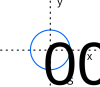
\includegraphics[scale=0.5]{s00}
\subsubsection{Pour l=1}
On dit qu'elles ont une symétrie de révolution autour d'un certain axe
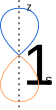
\includegraphics[scale=0.3]{s10}
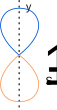
\includegraphics[scale=0.3]{s-11}
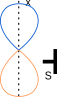
\includegraphics[scale=0.3]{s+11}
\subsubsection{Pour l=2}
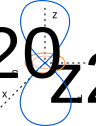
\includegraphics[scale=0.3]{s20}
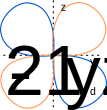
\includegraphics[scale=0.3]{s-21}
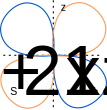
\includegraphics[scale=0.3]{s+21}
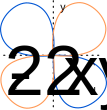
\includegraphics[scale=0.3]{s-22}
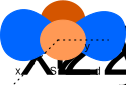
\includegraphics[scale=0.3]{s+22}
\end{document}

